\section{Equilibrated MD}

Molecular orientation analyses were performed to characterize the net molecular orientation of \wat~and \suldiox~molecules in the different locations near and within the water surface. Histograms were created to show the angles $\theta$ and $\phi$ relative to positions from the top surface of the aqueous slab. Both \wat~and \suldiox~orientations are considered for both the neat-\wat~and saturated systems.

\subsection{\wat~Orientation}

The results of the analyses for \wat~are shown in figure \ref{fig:water-orientation} for both the neat-water and saturated systems during the equilibrated MD simulations. In both systems an orientational preference is found at the slab surfaces where the water is in contact with the gas phase, or the surface \suldiox~molecules. The histograms are arranged with the plots of $\theta$ on the left and $\phi$ on the right columns, and the results for the neat-water and saturated systems are in the top and bottom rows, respectively. The distance axis was shifted such that the top surface is located at 0\angs, and the bottom surface is approx. 30\angs below. It is also noted that $\theta$ values of the bottom surface are inverted with respect to the top surface and should mirror those results. %The bisector tilt concentrates around $\cos(\theta)=0$ within the first few\angs of the surface, and then the distribution becomes isotropic further into the water bulk. As the tilt nears $\cos(\theta)=0$ the \wat~bisector lies within the plane of the surface indicating a water orientation either flat on the surface, or with some amount of ``twist'' sending the OH bonds in towards, or out of the bulk. The value of $\phi$ determines the ``twist'' in this case. Both systems show a peak in the distributions around $\cos(\phi)=1$ at the water surfaces. This results from an orientation of the water's y-axis (normal to the molecular plane) aligned perpendicular to the plane of the water surface.

The histograms show overall similarities for both systems in their shapes and intensities. The presence of a saturated layer of adsorbed \suldiox~molecules alters the water orientation, but not necessarily the location depth of the interface. In both $\theta$ distributions, the orientations of waters in the bulk region are isotropic until 5\angs below the surface location. At 5\angs below the surface the water molecules begin to orient with their bisectors within the plane of the interface (perpendicular to the surface normal, $\cos(\theta)\approx 0$). The corresponding location in the plot of $\phi$ shows that those molecules are also mostly flat to the surface ($\cos(\phi)\approx 1$). Moving further out from the bulk and into the gas phase, the distributions show $\cos(\theta)$ increasing. Waters further out from the bulk have fewer bonding interactions, and orient with their hydrogens more towards the gas phase. The bisector pointing further into the gas phase leads to isotropy in the values of $\phi$.  

The change in $\cos(\theta)$ is not as rapid at the neat-water surface as in the saturated system. Furthermore, the noise in the distribution above 5\angs (and below approx -34\angs) in the neat-water system is a result of fewer waters venturing beyond those extents and thus less data far from the surface. This is one indication that waters near a layer of adsorbed \suldiox~venture further above the interface and interact with the \suldiox~molecules. The interactions with neighboring \suldiox~molecules allow the waters above the surface to orient more perpendicular to the interface. Recent SFG studies by our group indicate that ***<something goes here>***.

The distribution of $\cos(\phi)$ is more sharply defined (i.e. less isotropic) for the neat-water system than for the saturated one. Waters on the neat surface lie flatter, whereas the presence of the \suldiox~allows a greater range of ``twist'' for those waters in the plane of the interface. The $\phi$ distributions quickly become isotropic above a couple angstroms from the surface as the bisectors orient perpendicularly, and below the surface as the bulk water loses any orientational preference.

%Peaks in the distributions of the neat-\wat~system are more clearly pronounced as their intensities are more concentrated and larger than the surrounding area of the profiles. This difference indicates that the transition from the preferred orientation at the water surface has a sharper distinction from the isotropic bulk than in the system with the saturated \suldiox~surface. It appears that the same orientation trend is present in both systems, but the presence of the \suldiox~at the water surface decreases the degree of water orientation at the interface.

\begin{figure}[h!]
	\begin{center}
		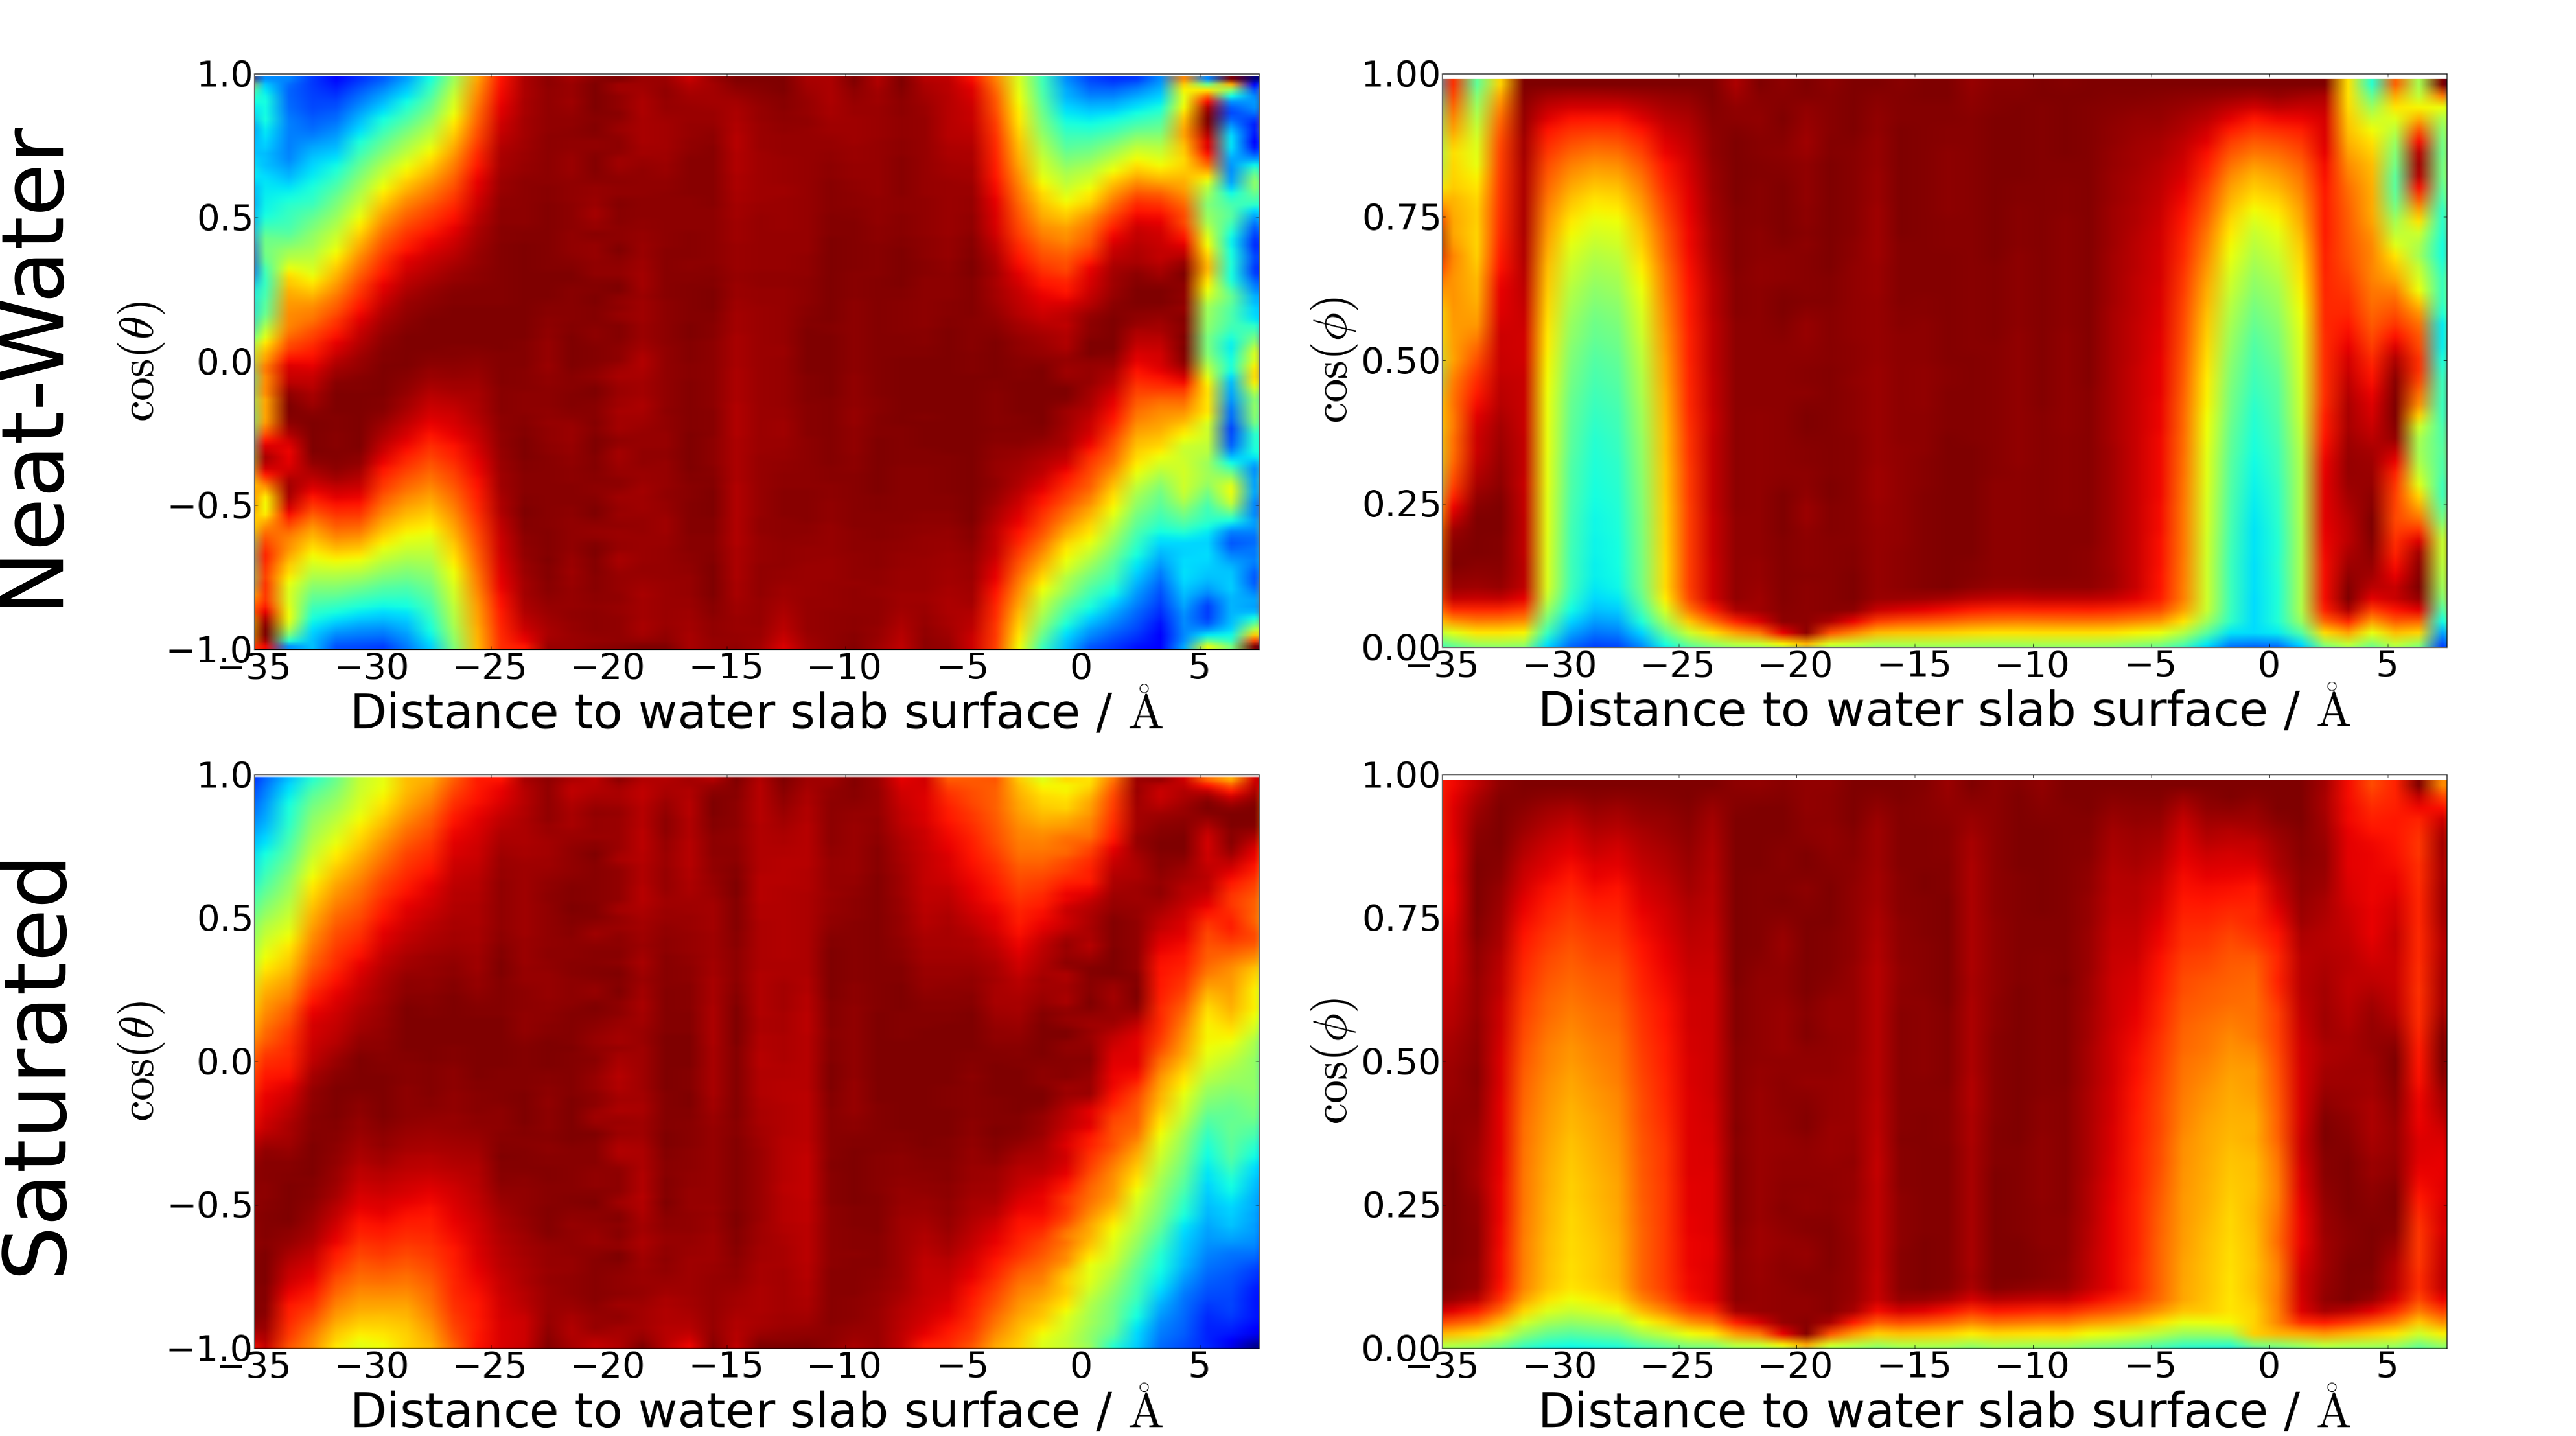
\includegraphics[scale=1.0]{images/h2o-angles/h2oangles.png}
		\caption{Molecular orientation histograms of \wat~throughout the surface equilibrated systems. The top surface is located at a distance of 0 with negative positions in the bulk of the slab. The bottom slab surface is approx. 30\angs below the top surface. Shown are the angle distributions for $\theta$ (left column) and $\phi$ (right column) in both the neat-\wat~system (top row) and the saturated system (bottom row). The distributions are normalized to account for the changing number of water molecules at different positions in the system.}
		\label{fig:water-orientation}
	\end{center}
\end{figure}



\subsection{\suldiox~Orientation}

Orientation distributions of the adsorbed \suldiox~molecules were created during the equilibrium simulations for both the neat-\wat~and saturated \suldiox~systems. Figure \ref{fig:so2-orientation} shows the distributions of $\cos(\theta)$ and $\cos(\phi)$ (arranged similar to the water orientation distributions plots in figure \ref{fig:water-orientation}). The data set for the neat-\wat~system is much smaller as only a single \suldiox~molecule was simulated in the bulk. The resulting distribution plots are thus noisier than the corresponding saturated plots, but effective comparisons can still be drawn.

The location of \suldiox~within the water surface is slightly different between the two equilibrium MD systems (see figure \ref{fig:density}). The single \suldiox~molecule is generally located just below the 0\angs position of the surface, and the distribution of the concentrated system \suldiox~molecules is centered above the surface location. This indicates that in both systems the \suldiox~is highly surface active, but the locations of the peak \suldiox~densities differ. The single molecule spends most of its time bound within the top water monolayer, and often traversing below that location by only a few\angs. The saturated system's surface molecules sit on top of the monolayer. The angular distribution of the single \suldiox~is concentrated primarily in $\cos(\theta)>0$, such that the bisector points out of the water surface. This same distribution occurs in the saturated system for positions below 0\angs, but the orientation becomes isotropic for molecules located above 0\angs, on top of the water surface. Promixity to the water highly orients the \suldiox~with the sulfur atom pointing in towards the water bulk.

\begin{figure}[h!]
	\begin{center}
		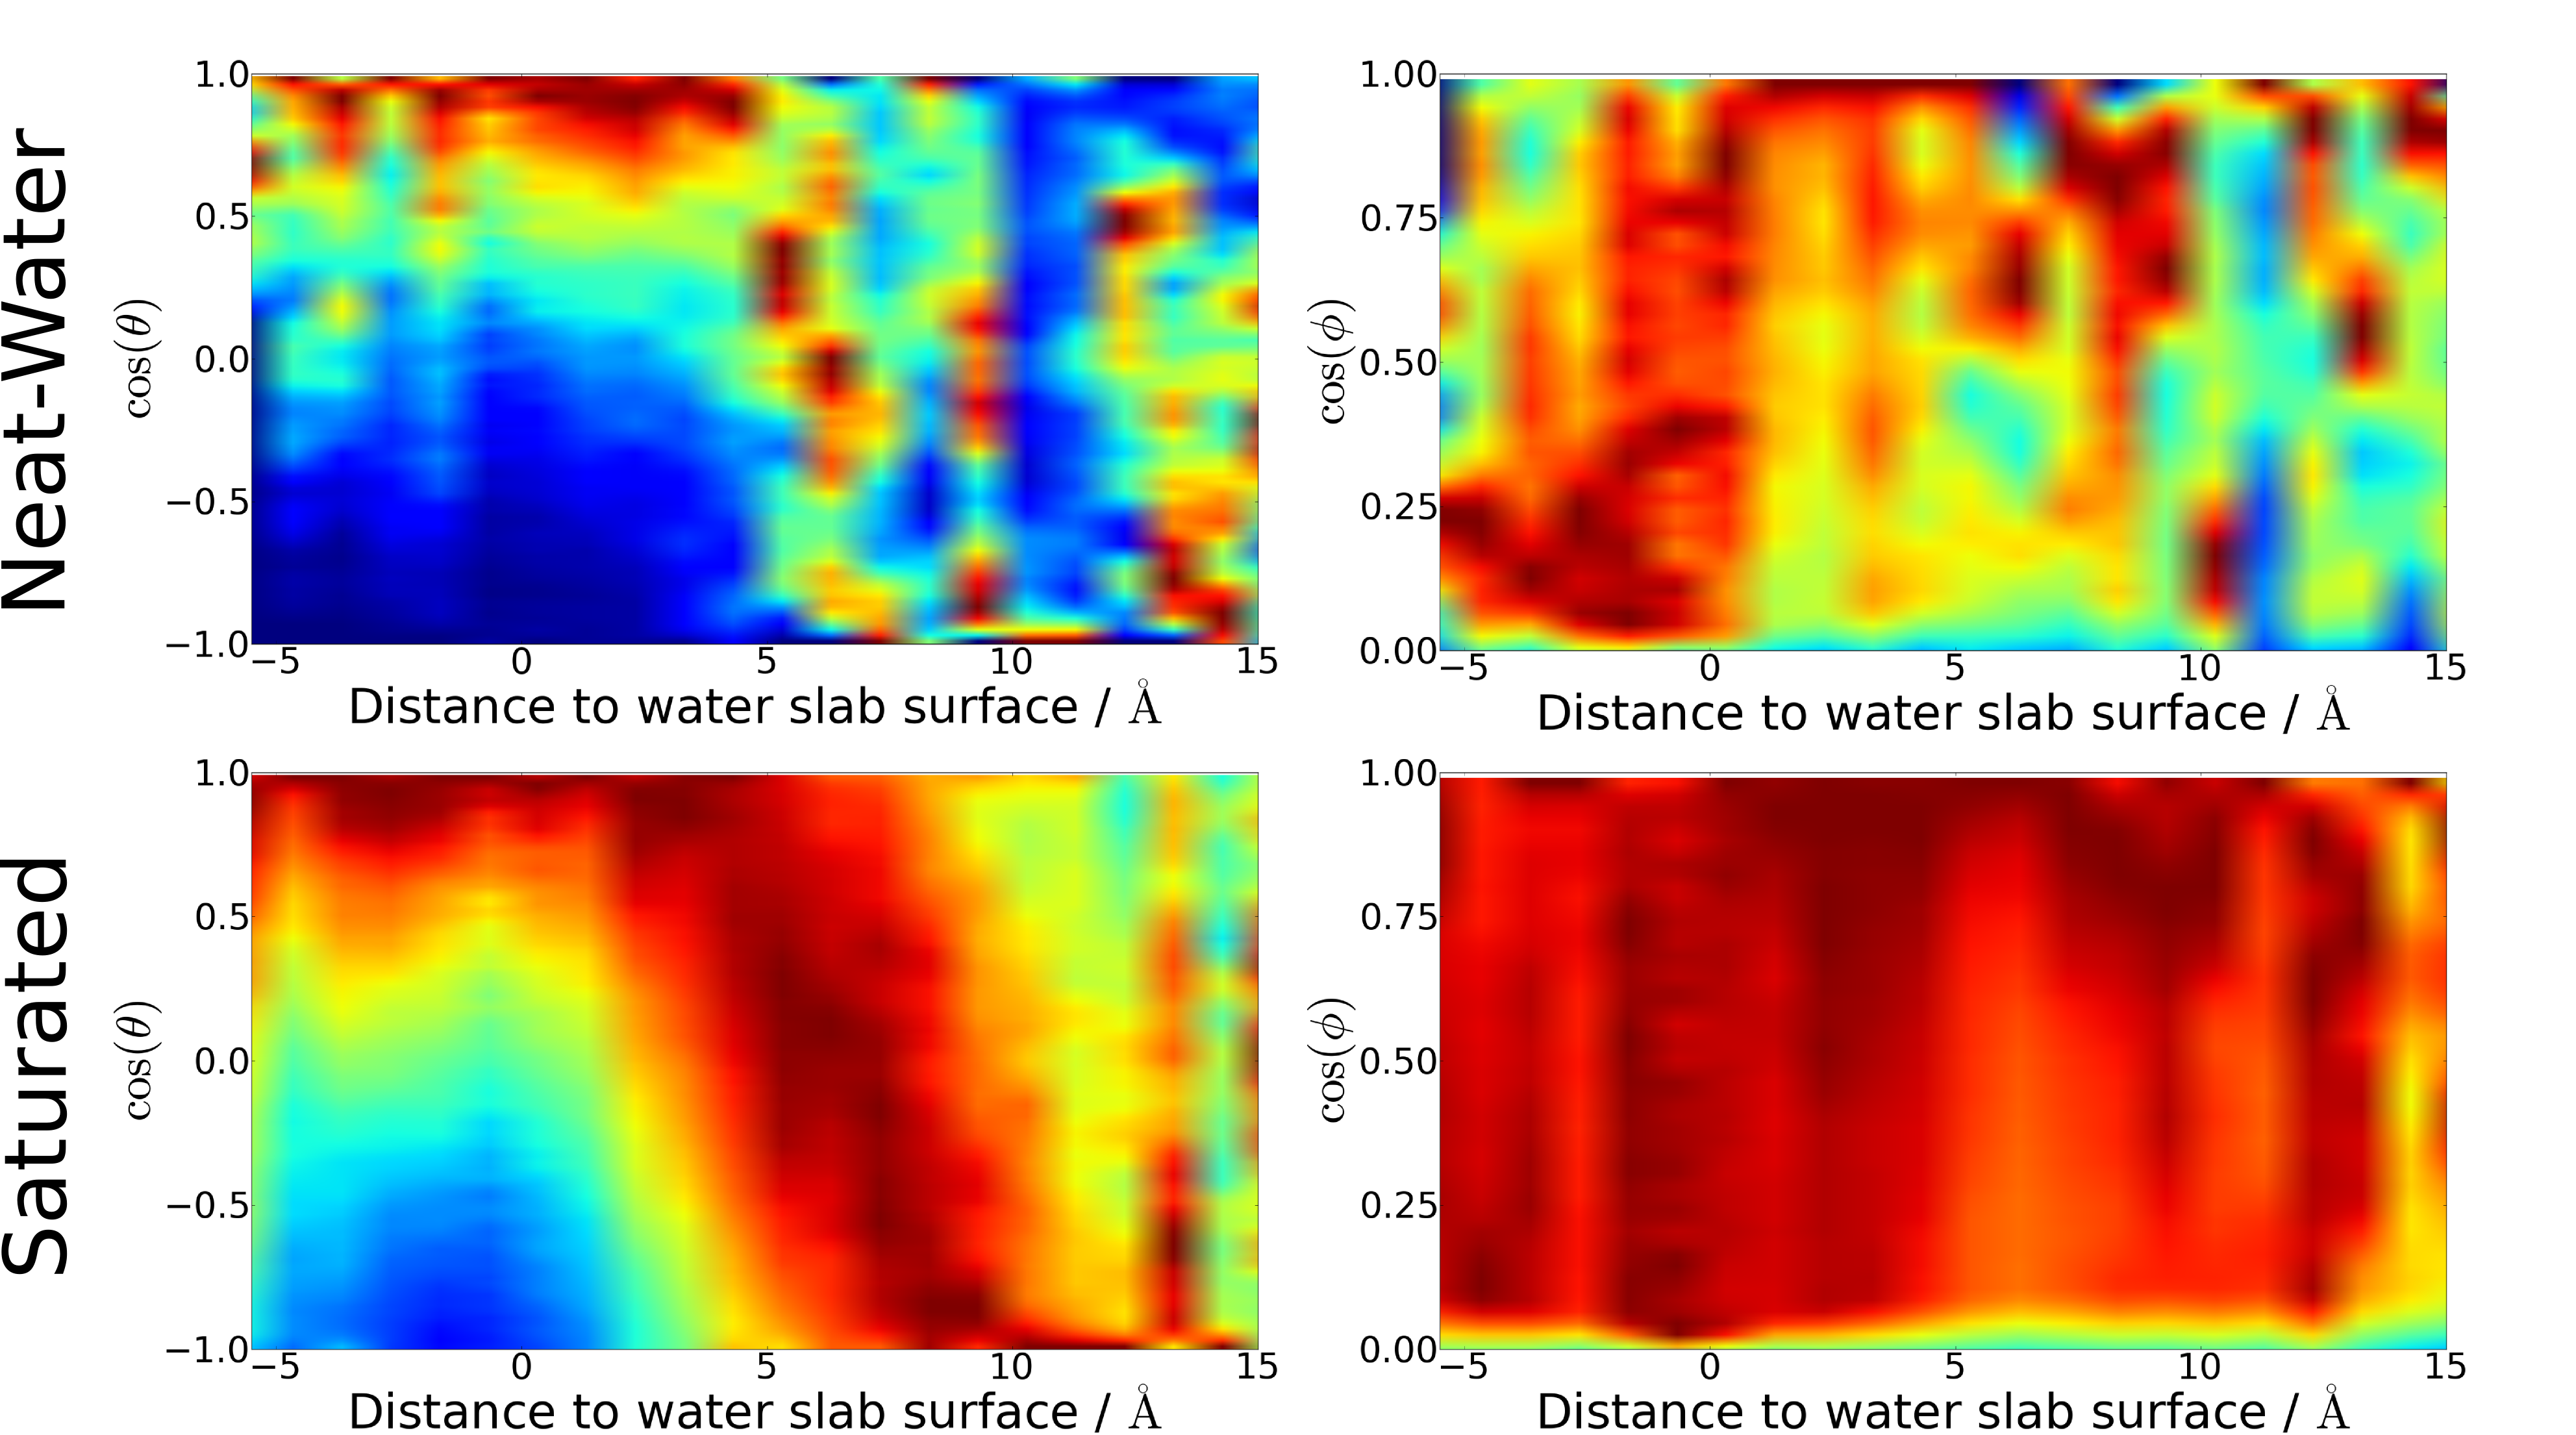
\includegraphics[scale=1.0]{images/so2-angles/so2-angles.png}
		\caption{Molecular orientation distributions for \suldiox~molecules adsorbed to the water slab surface. Distributions are shown for $\cos(\theta)$ (left column) and $\cos(\phi)$ (right column) for both the neat-\wat~(top) and high \suldiox~concentration (bottom) systems. For both systems the $\theta$ distributions suggest \suldiox~bound to the water surface with the sulfur pointing towards the water slab, and the oxygens pointing to the gas phase. In this configuration the $\phi$ distribution is isotropic because of the water slab's in-plane symmetry.}
		\label{fig:so2-orientation}
	\end{center}
\end{figure}
